\section{实验过程}
实验的主要过程是特征提取,也比较了不同分类器的分类结果。
实验过程是递进式的,即在上一次实验的结果上,考察新的特征提取技术,看对于最终的分类结果有没有帮助。\\
\subsection{分类结果评价标准}
实验使用ROC曲线和AUC值作为分类结果的评价标准。\\
ROC空间将假阳性率FPR作为X轴,真阳性率TPR作为Y轴。
我们研究的情感分析是一个二元分类问题。
利用分类器作二元的概率预测,然后在不同的阈值条件下,可以得到不同的FPR和TPR。
将FPR和TPR对应的$ (x, y) $ 座标点拟合成一条曲线,就是ROC曲线。\\
而AUC就是ROC曲线下面积,其直观的含义是:如果随机抽取一个阳性样本和一个阴性样本,分类器正确判断阳性样本的值高于阴性样本的概率。
从AUC值可以直观地判断分类器的表现。
\begin{itemize}
	\item
	  $ AUC = 1 $:是一个完美分类器,意味着存在至少一个阈值能得到完美的预测。不过在绝大多数的预测场合,不存在完美分类器。
	\item
	  $ 0.5 < AUC < 1 $:分类器优于随机猜测,选择一个妥善的阈值,有预测价值。
	\item
	  $ AUC = 0.5 $:随机猜测模型,没有预测价值。
	\item
	  $ AUC < 0.5 $:分类器比随机预测结果还要差,但是只要预测结果取反,就优于随机猜测。
\end{itemize}
也就是说,如果分类器的AUC值越大,其性能越好。

\subsection{训练集、测试集分割}
训练集和测试集的分割基于“二八”原则,即采用原始数据集的$ 80\% $作为训练集,$ 20\% $作为测试集。\\
同时为了防止训练集过小产生过拟合现象,我们使用交叉验证的方式来分割原始数据集。
实验中使用K次交叉验证的方式。
所谓K次交叉验证,是指将原始数据集分割成K个子样本,一个单独的子样本被保留作为测试集,其他$ K-1 $个样本用来训练。
交叉验证重复K次,每个子样本验证一次,平均K次的结果,得到一个单一的预测。
K次交叉验证的好处在于可以同时重复使用随机产生的子样本进行训练和验证,每次的结果验证一次。

\subsection{基于词包的特征提取}
将词包作为文本的特征是一个经典,简单直观而有效的特征提取方式,课上也讲过这个方法。
在词包模型中,文本被表示成组成它的词的包(多重集合)。
这个集合保留了词的重复次数,但是忽略文本的语法和词之间的顺序。\\
词包模型首先构建文本的词汇表,然后取最频繁的词汇作为词包的考察元素。
对于每个文本,统计各个频繁词的出现次数,作为该段文本的特征。\\
举例来讲,我们有两段文本:
\begin{itemize}
	\item
	``John likes to watch movies. Mary likes movie too.''
	\item
	``John also likes to watch football games.''
\end{itemize}
由这两段文本构造的词包为:
[ "John", "likes", "to", "watch", "movies", "also", "football", "games", "Mary", "too"]。
有了词包之后,我们就可以来构造文本的特征了。
最常用的方式是词汇频数。
上述例子构造的文本特征为:
\begin{itemize}
	\item
	``[1, 2, 1, 1, 2, 0, 0, 0, 1, 1]''
	\item
	``[1, 1, 1, 1, 0, 1, 1, 1, 0, 0]''
\end{itemize}

将词包作为文本的特征是一个经典,简单直观而有效的特征提取方式,课上也讲过这个方法。
在词包模型中,文本被表示成组成它的词的包(多重集合)。
这个集合保留了词的重复次数,但是忽略文本的语法和词之间的顺序。\\
词包模型首先构建文本的词汇表,然后取最频繁的词汇作为词包的考察元素。
对于每个文本,统计各个频繁词的出现次数,作为该段文本的特征。\\
举例来讲,我们有两段文本:
\begin{itemize}
	\item
	  ``John likes to watch movies. Mary likes movie too.''
	\item
	  ``John also likes to watch football games.''
\end{itemize}
由这两段文本构造的词包为:
[ "John", "likes", "to", "watch", "movies", "also", "football", "games", "Mary", "too"]。
有了词包之后,我们就可以来构造文本的特征了。
最常用的方式是词汇频数。
上述例子构造的文本特征为:
\begin{itemize}
	\item
	  ``[1, 2, 1, 1, 2, 0, 0, 0, 1, 1]''
	\item
	  ``[1, 1, 1, 1, 0, 1, 1, 1, 0, 0]''
\end{itemize}

\subsubsection{简单词包}
我们采用scikit-learn提供的词包模块(sklearn.feature\_extraction.text.CountVectorizer)来计算文本的词包特征。\\
我们抽出训练集词包中的前几个词: ['abandoned',
'abc',
'abilities',
'ability',
'able',
'abraham',
'absence',
'absent',
'absolute',
'absolutely'
]。\\

提取出特征后,使用了三种分类器:
\begin{itemize}
	\item
	  随机森林模型  \\
	  (sklearn.ensemble.RandomForestClassifier)
	\item
	  高斯朴素贝叶斯模型  \\
	  (sklearn.naive\_bayes.GaussianNB)
	\item
	  线性回归模型  \\
	  (sklearn.linear\_model.LogisticRegression)
\end{itemize}
三种分类器的分类结果如下图所示(图\ref{fig:rfroc}, 图\ref{fig:gnbroc}, 图\ref{fig:lrroc}, 图\ref{fig:3croc}),我们以ROC和AUC作为评价结果。
\begin{figure}[h]
\centering
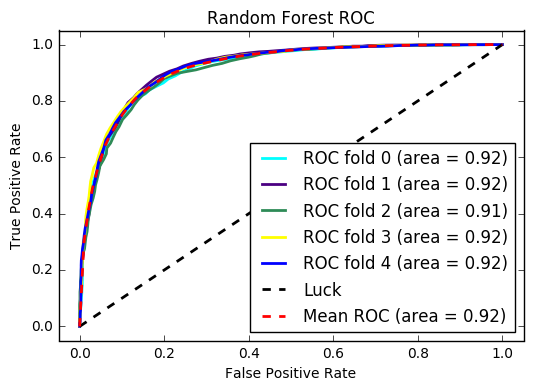
\includegraphics[width=0.9\linewidth]{rf_roc}
\caption[rf_roc]{随机森林模型交叉验证的ROC曲线}
\label{fig:rfroc}
\end{figure}

\begin{figure}[p]
\centering
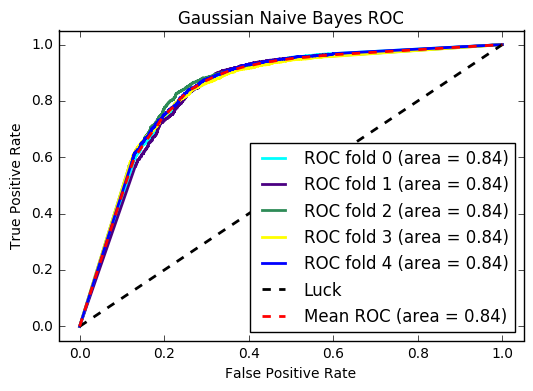
\includegraphics[width=0.9\linewidth]{gnb_roc}
\caption[gnb_roc]{高斯朴素贝叶斯模型交叉验证的ROC曲线}
\label{fig:gnbroc}
\end{figure}

\begin{figure}[p]
\centering
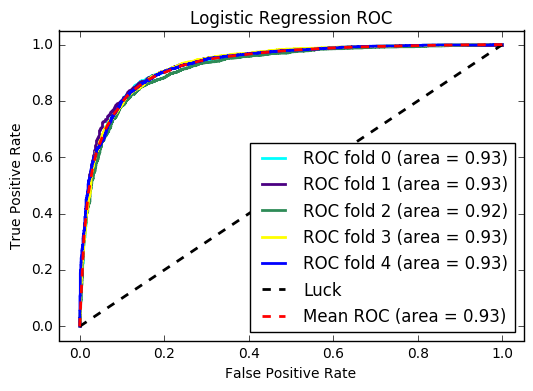
\includegraphics[width=0.9\linewidth]{lr_roc}
\caption[lr_roc]{线性回归模型交叉验证的ROC曲线}
\label{fig:lrroc}
\end{figure}

\begin{figure}[p]
\centering
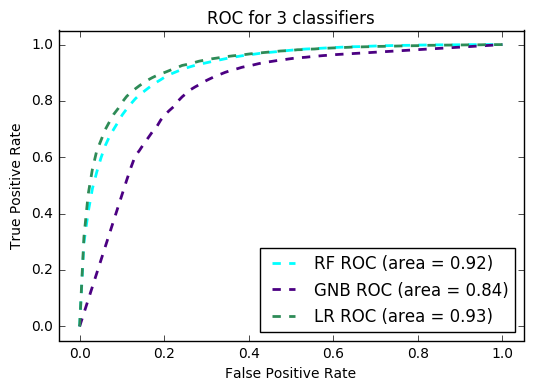
\includegraphics[width=0.9\linewidth]{3c_roc}
\caption[3c_roc]{三种模型的平均ROC曲线}
\label{fig:3croc}
\end{figure}

从三种分类器的K次交叉验证绘制出的ROC曲线来看,各个交叉验证集的ROC曲线几乎完全重合,似乎没有必要对这个数据集进行交叉验证。
另一方面,我们在实验中使用了5次交叉验证,也就是说训练时间比单个训练集测试集的方式多了4倍。
从性能和运行效率的角度考虑,我们在之后的实验中不再进行交叉验证,以节省时间。\\
在三种分类模型的横向比较中,我们发现训练过程中,随机森林的训练时间 > > 线性回归模型 > 高斯朴素贝叶斯模型。
而随机森林模型和线性回归模型的分类性能相差不大。
\paragraph{简单词包的问题}

\paragraph{简单词包的问题}
\begin{itemize}
	\item
	简单词包的方法忽略了词之间的位置关系,而只计算了词的频数。
	这样的方式缺失了上下文信息,提取的是孤立的特征。
	\item
	简单词包的方法将词包中所有的词一视同仁,没有考虑到有些词比较重要,而另一些词不是那么重要。
\end{itemize}
\paragraph{改进方式}
\begin{itemize}
	\item
	针对第一个问题,我们采用课上学到的”n-gram"的思想,将原始数据集先提取出bi-gram的特征,然后对这些特征作词包。
	\item
	针对第二个问题,我们计算文本词汇的“TF-IDF”值,作为词包集合中元素的加权值,然后将加权后的特征作为训练集测试集。
\end{itemize}

\subsubsection{基于bigram的词包}
n-gram的模型特征可以作为文本的空间信息特征。
我们仍然使用scikit-learn的CountVectorizer模块来提取词包特征,不过这时的ngram\_range参数为(2, 2),表示我们使用bigram作为词包的基本单元。\\
我们抽出前几个bigram特征:['able get',
'able make',
'able see',
'able watch',
'absolute worst',
'absolutely brilliant',
'absolutely hilarious',
'absolutely love',
'absolutely loved',
'absolutely nothing'] \\
从这几个bigram特征可以预见到提取出的特征词包中有很多像副词那样的修饰词。\\
将提取到的bigram词包特征用来训练分类器模型,得到如下图所示的ROC曲线。
\begin{figure}[h]
\centering
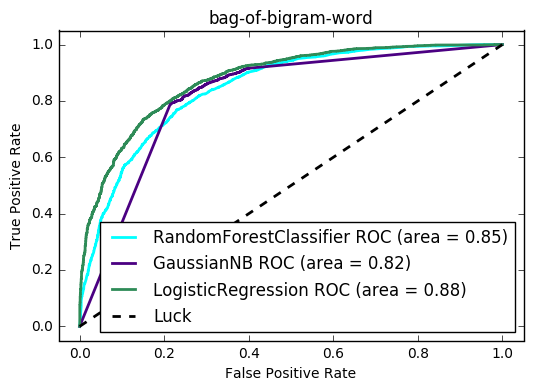
\includegraphics[width=0.9\linewidth]{3c_roc_bigram}
\caption[3c\_roc\_bigram]{三种模型用bigram词包的ROC曲线}
\label{fig:3crocbigram}
\end{figure}
从大体上我们可以看到,使用了bigram特征的分类器,其整体性能都比不使用bigram特征的分类器要差。
究其原因,我认为是像'absolutely'这样的副词修饰词占用了太多特征位置,导致其他一个词的强调词(或者那类一个词就可以鲜明地表达态度的词)没有成为词包中的频繁词,从而缺失了更有意义的特征。

从基于bigram的词包进行分类的结果来看,我们对于这个数据集倾向于不使用bigram词包,而是继续使用简单的unigram词包。

\subsubsection{基于TF-IDF的加权词包}
简单地计算词汇的频数不见得是最好的特征提取方式,尽管我们已经去除了停用词,但是文本中仍然会存在有些词比其他词更重要。
词的重要性随着它在文本中出现的次数成正比增加,但同时又随着它在语料库中出现的频率成反比下降。\\
使用TF-IDF作为词重要性的考核标准是因为:如果一个词在一段文本中出现的频率TF高,并且在其他文本中很少出现,那么我们就认为这个词具有很好的类别区分能力,适合用来分类。\\
词频(term frequency, TF)是指某个词在文本中出现的频率。
对文本$ j $里的词$ t_i $来说,其TF计算方式如下\ref{tf}:
\begin{equation}\label{tf}
  TF_{i, j} = \frac{n_{i, j}}{\sum_{k}n_{k, j}}
\end{equation}
其中$ n_{i, j}$是该词在文本 $ d_j $中出现的次数,而分母则是在文本$ d_j $中所有词出现的次数和。\\
逆向文件频率(inverse document frequency, IDF)是对一个词普遍重要性的度量。
某一个词的IDF,可以由总文本数目除以包含该词的文件的数目,再将得到的商去对数可得。
IDF的计算方式如下\ref{idf}:
\begin{equation}\label{idf}
  IDF_i = \log\frac{{| D |}}{| \{ j: t_i \in d_j \} | + 1}
\end{equation}
其中$ | D | $ 是语料库中的文本总数,$ | \{ j : t_i \in d_j \} | $是包含词 $ t_i $文本数目。\\
由TF和IDF可得TF-IDF的计算方法\ref{tfidf}:
\begin{equation}\label{tfidf}
  TFIDF_{i, j} = TF_{i, j} * IDF_{i}
\end{equation}
某个词在某一文本中的高词语频率,以及该词在这个文本集合中的低文本频率,可以产生出高权重的TF-IDF。
因此,TF-IDF倾向于过滤掉常见的词语,保留重要的词语。\\
我们使用scikit-learn提供的TfidfVectorizer模块(sklearn.feature\_extraction.text.TfidfVectorizer)来计算词汇的TF-IDF值,得到和CountVectorizer计算结果一样大小的矩阵,然后将这两个矩阵按元素相乘,得到词包的TF-IDF加权特征。
以这个特征集合来训练分类器,得到如下图\ref{fig:3croctfidf}所示的ROC曲线。
\begin{figure}[h]
\centering
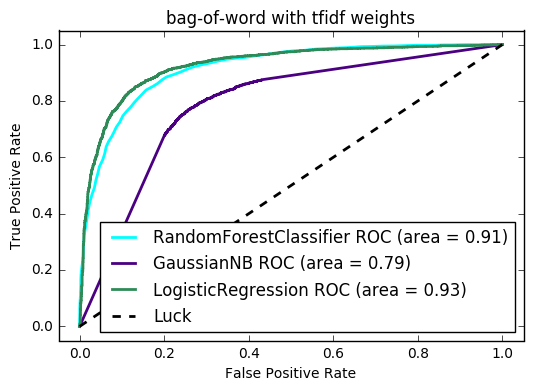
\includegraphics[width=0.9\linewidth]{3c_roc_tfidf}
\caption[roctfidf]{三种模型用TF-IDF加权词包的ROC曲线}
\label{fig:3croctfidf}
\end{figure}

从图中可以看出,这个结果和图4的简单词包的ROC曲线在误差范围内差异不大,但是高斯朴素贝叶斯模型的AUC值却有明显差距。
对于这个差异,我也不是很理解,留待进一步的研究。\\

从基于TF-IDF的加权词包进行分类的结果来看,似乎文本语料库中没有哪些词是特别突出的。
也可以理解为大家在评论电影时,不会趋向于使用其他人听不懂或者不了解的词汇,而是会在一套共通的话语体系下作评论。
从这个角度来理解的话,那TF-IDF加权在这里并没有多大的作用。

\subsection{基于词向量的特征提取}
基于词包的特征提取有一个明显的问题,那就是它只是作生硬的词汇统计,而没有尝试去理解文本的意思。
针对这个问题,我们尝试另一种提取特征的方式——词向量。\\
词向量(Word2vec)最早是由Google的研究人员提出。
词向量模型是一个两层的神经网络模型,通过训练这个神经网络来重构词的上下文语义。\\
词向量模型需要一个很大的文本语料库作为训练集,然后生成一个几百维度的向量空间。
在这个向量空间中,语料库的每个词都有一个对应的向量。\\
 词向量模型有一个明显的优点,那就是它可以理解上下文的语义。
 因为一个词现在可以认为是高维向量空间中的一个点,而有着相似上下文语义的词,他们在向量空间中的位置也很接近。
 也就是说,有着相似意思的词在空间中聚合成簇。
 这样,通过考察词向量的位置,词与词之间的空间距离,利用向量运算,我们就可以构造出能够理解语义的特征集。\\
 词向量模型有一个生动的例子来表示该模型对于语义理解的能力:“king" - "man" + "woman" = "queen"。
 这个例子表明词向量可以理解"king"和"queen"之间的差异,以及两者之间的转换方式(-"man" + "woman")。\\
 尽管之前也有利用神经网络(如深度神经网络,卷积神经网络)来学习文本词特征表示的,但是这些方法都需要长时间的模型训练,对硬件的要求也很高(通常需要GPU加速),这对于个人的课程项目实验来说是不切实际的。
 因此我们在这里选择使用词向量模型,它的学习速度相对其他神经网络模型来说快得多。
 
 \subsubsection{训练词向量模型}
训练词向量模型并不需要监督学习,而为了达到最好的学习效果,我们要提供尽可能丰富的语料作为训练集,因此我们使用所有的电影评论语料(不管有没有打标签)作为词向量模型的训练集。\\
基于同样的理由,我们在清洗原始数据集作为语料库时,将不去除停用词。
这样训练网络可以获得更丰富的文本,从而得到更高质量的词向量空间。\\
我们使用gensim这个Python包来训练词向量,它提供了对词向量模型很好的实现。
同时使用Cython来加速Python的训练代码。
对于原始文本的分句工作,我们使用NLTK提供的punkt分词器。

 
 \subsubsection{探索词向量模型}
在上一步词向量模型训练完成后,我们来考察这个模型对于语义的理解。
首先来看看这个模型有没有区分不同语义实体的能力,探索结果如图\ref{fig:doesntsimilar}:
\begin{figure}[h]
\centering
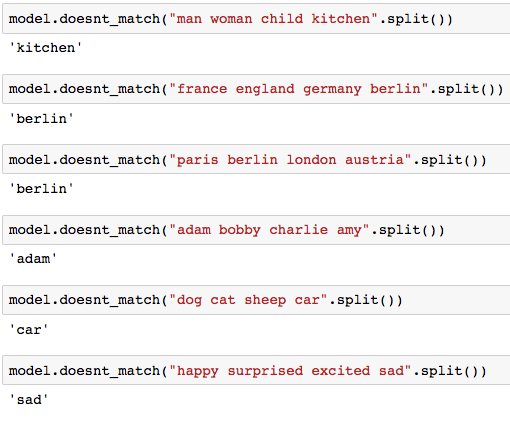
\includegraphics[width=0.9\linewidth]{doesnt_similar}
\caption[doesnt_similar]{探索词向量区分语义实体的能力}
\label{fig:doesntsimilar}
\end{figure}
从探索结果中可以看出,该模型对于语义实体的区分能力很不错。\\
之前也介绍说词向量模型可以通过向量空间距离关系来查找相似词,我们的探索结果如图\ref{fig:similar1}、图\ref{fig:similar2}、图\ref{fig:similar3}:
\begin{figure}[h]
\centering
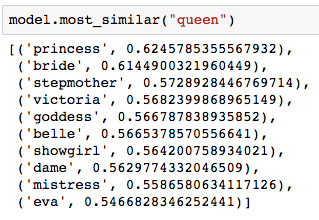
\includegraphics[width=0.8\linewidth]{similar1}
\caption[similar1]{探索词向量查找相似词的能力1}
\label{fig:similar1}
\end{figure}
\begin{figure}[h]
	\centering
	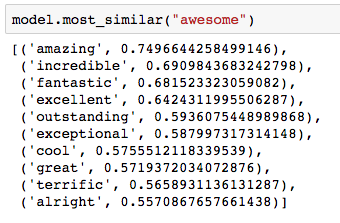
\includegraphics[width=0.8\linewidth]{similar2}
	\caption[similar2]{探索词向量查找相似词的能力2}
	\label{fig:similar2}
\end{figure}
\begin{figure}[h]
	\centering
	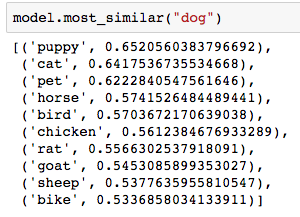
\includegraphics[width=0.8\linewidth]{similar3}
	\caption[similar3]{探索词向量查找相似词的能力3}
	\label{fig:similar3}
\end{figure}

从这几个探索的结果看来,词向量模型能够很好地查找出具有相似语义的词。
而这个相似不只是意思上的相似,还有语义实体在人类认知世界中概念分类上相似,如探索结果3,图\ref{fig:similar3}),相似词都是动物,更具体点是家畜类,而探索结果1,图\ref{fig:similar1},相似词都是女性角色。\\
从模型探索的结果来看,词向量模型弥补了词包模型对于语义理解的缺失,可以为特征提取工作提供更多有上下文含义的特征。\\
 
 在训练完词向量模型之后,我们要使用这个词向量模型来构造评论语料库的特征。
 
 \subsubsection{向量平均}
由之前的介绍可知,词向量模型中,每个词都是一个高维向量,那么最简单直接的构造特征的方式就是将一段文本中所有词的词向量相加取平均,得到这段文本的平均词向量,将这个平均词向量作为该段文本的特征集合。\\
从直观角度理解,这种方式就是将一段文本的“重心”作为该段文本的特征。\\
利用这种特征来训练分类器,得到如下图\ref{fig:3cword2vecaverage}所示的ROC曲线。
\begin{figure}[h]
\centering
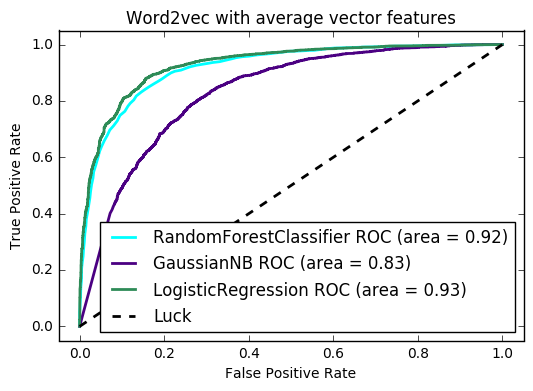
\includegraphics[width=0.9\linewidth]{3c_word2vec_average}
\caption[word2vec_average]{三种模型用Word2vec的平均词向量特征的ROC曲线}
\label{fig:3cword2vecaverage}
\end{figure}
用这个结果和简单词包的图4比较,发现在误差允许范围内,这种方式对结果并没有什么提高。\\
猜测原因是因为词向量虽然提供了文本的语义信息,但是却丢失了文本的统计信息。
从这个结果可以看出,词向量特征和词包特征是一对互补的特征,前者提供了语义信息,后者提供了统计信息。\\